\documentclass[12pt,a4paper,twopage]{article}
\usepackage[utf8]{inputenc}
\usepackage[a4paper,margin=1cm,footskip=.5cm]{geometry}
\usepackage{multicol}
\usepackage{amsmath}
\usepackage{float}
\usepackage{epsfig,graphicx}
\usepackage{xcolor,import}
\usepackage{subcaption}
\usepackage[font=small,labelfont=bf]{caption}
\usepackage{siunitx}
\usepackage[german]{babel}
\usepackage{textcomp}
\usepackage{mathtools}
\linespread{1.1}
\usepackage{parskip}
\setlength{\parindent}{12pt}

\begin{document}


\thispagestyle{empty}
			\begin{center}
			\Large{Fakultät für Physik}\\
			\end{center}
\begin{verbatim}


\end{verbatim}
							%Eintrag des Wintersemesters
			\begin{center}
			\textbf{\LARGE SOMMERSEMESTER 2015}
			\end{center}
\begin{verbatim}


\end{verbatim}
			\begin{center}
			\textbf{\LARGE{Physikalisches Praktikum II}}
			\end{center}
\begin{verbatim}




\end{verbatim}

			\begin{center}
			\textbf{\LARGE{PROTOKOLL}}
			\end{center}
			
\begin{verbatim}





\end{verbatim}

			\begin{flushleft}
			\textbf{\Large{Experiment (Nr., Titel):}}\\
			PS9, Heißluftmotor - Stirlingprozess
							%Experiment Nr. und Titel statt den Punkten eintragen
			\LARGE{}	
			\end{flushleft}

\begin{verbatim}

\end{verbatim}	
							%Eintragen des Abgabedatums, oder des Erstelldatums des Protokolls
			\begin{flushleft}
			\textbf{\Large{Datum:}} \Large{29.5.2015}
			\end{flushleft}
			
\begin{verbatim}
\end{verbatim}
							%Namen der Protokollschreiber
		\begin{flushleft}
			\textbf{\Large{Bachleitner Veronika, Grafendorfer Erik}} 
			\end{flushleft}

\begin{verbatim}


\end{verbatim}
							%Kurstag und Gruppennummer, zb. Fr/5
			\begin{flushleft}
			\textbf{\Large{Kurstag/Gruppe:}} \Large{FR/1}
			\end{flushleft}

\begin{verbatim}






\end{verbatim}
							%Name des Betreuers, das Praktikum betreute.
			\begin{flushleft}
			\LARGE{\textbf{Betreuer:\Large{ }}}		
			\end{flushleft}
			
\section{Aufgabenstellung}

\section{Theorie}
\subsection{Allgemeine Grundlagen}
Die drei Hauptsätze der Wärmelehre bilden die Grundlage für die folgenden Experimente:\\
1. Wärme ist eine Form von Energie: und zwar die thermische Energie, die in der ungeordneten Bewegung der Atome / Moleküle eines Stoffes gespeichert ist.\\
2. Wärme geht nur von einem Körper höherer Temperature auf einen niedrigerer Temperatur über. ($\Delta S \geq 0$, $S$ die Entropie).\\
3. Der absolute Nullpunkt kann nicht erreicht werden.\\
\\
Wärme kann über Wärmeleitung, Strahlung und Konvektion übertragen werden.\\
\\
\textbf{Wärmeleitung} ist vor allem für Festkörper wichtig. Die Übertragung der Bewegungsenergie durch Leitungselektronen ist besonders wirksam, daher sind gute elektrische Leiter auch gute Wärmeleiter. In Isolatoren erfolgt die Übertragung nicht mittels Elektronen sondern über die Gitterschwingungen (Phononen), allerdings mit wesentlich geringerer Wirksamkeit.\\
\\
Die Bedeutung der \textbf{Strahlung} wird mit dem Stefan-Boltzmann-Gesetz gut erklärt: $p(T)=\sigma_{SB} T^4$. Man sieht hier die hohe Abhängigkeit von der Temperatur.\\
\\
\textbf{Konvektion} passiert in Flüssigkeiten und Gasen: Erwärmte Materie wird mit einer Strömung transportiert. Dieser Effekt spielt eine große Rolle bei Wetter, Klima, Heizungen, Energietechnik und vielen mehr. 

\subsection{Wärmeleitung in Metallen}
Den Zusammenhang zwischen Wärmeenergie $Q$ und Wärmestromdichte $\vec{q}$ gibt die Kontinuitätsgleichung:
$$\frac{\partial}{\partial t}\left(\frac{\partial Q}{\partial V}\right) + div \vec{q}=0$$
Die zeitliche Änderung der Wärmeenergie pro Volumen wird erfolgt also über einen Wärmestrom.\\
Daraus ergibt sich auch das 1. Fick'sche Gesetz:
$$\frac{\partial}{\partial V}\Phi + div \vec{q}=0$$
Außerdem gibt es noch das zweite Fick'sche Gesetz:
$$\frac{\partial T}{\partial t}-\frac{\lambda}{\rho c	}\frac{\partial^2 T}{\partial \vec{x}^2}=0$$
mit der Temperatur $T$, der Zeit $t$, der Wärmeleitfähigkeit $\lambda$, der Massendichte $\rho$ und der spezifischen Wärmekapazität $c$.

\subsection{Wärmeleitung in Isolatoren}

\section{Aufbau}

\section{Durchführung}
Die Wärmebildkamera hat eine Auflösung von 120x160 Pixel.

\section{Ergebnisse}
\subsection{Wärmeleitfähigkeit von Metallen}
\subsubsection{Nichtstationärer Wärmestrom}

\begin{figure}[H]
\centering
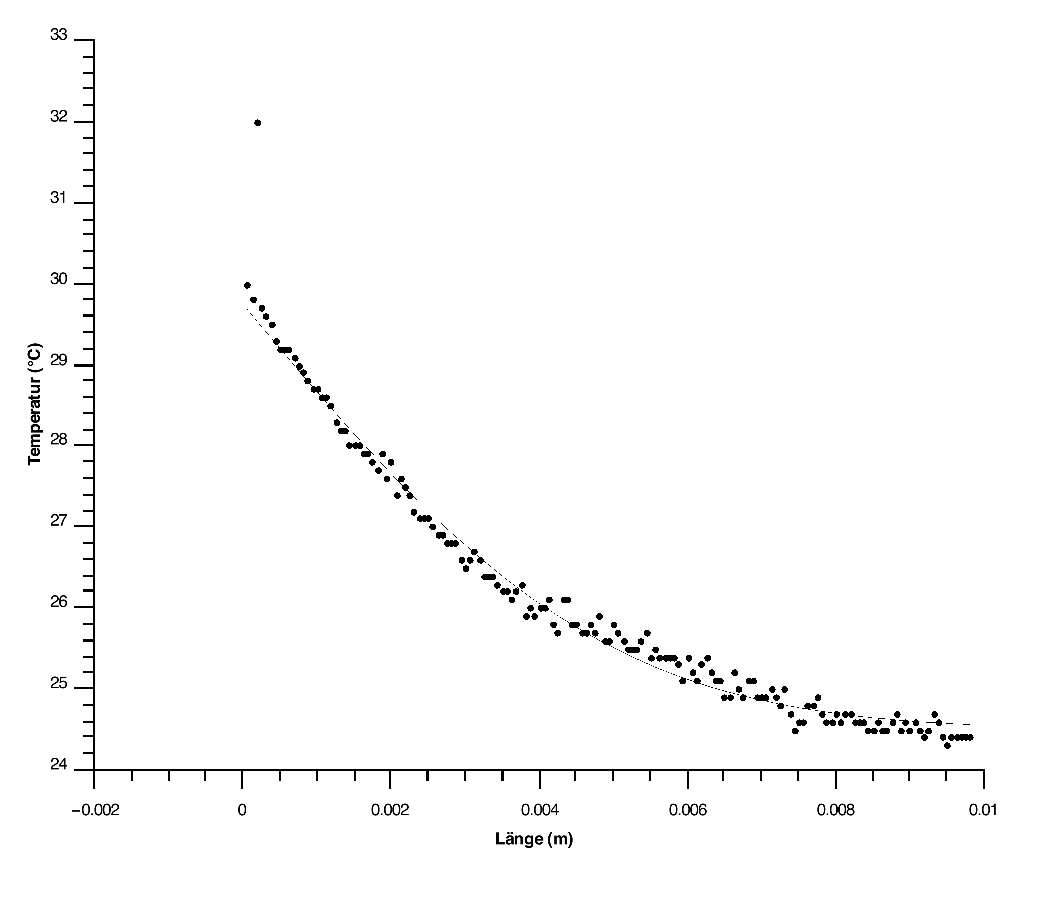
\includegraphics[scale=0.8]{nichtstationaer.eps}
\caption{Messung mit der Wärmebildkamera: Temperatur gegen Länge bei nichtstationärem Wärmestrom.}
\end{figure}

Wir verwenden zur Bestimmung der Wärmeleitfähigkeit folgende Gleichung:
$$T(x,t)=(T_0 - T_{max}) \cdot erf\left(\frac{1}{\sqrt{4\chi t}}x\right) + T_{max}$$
QTI-Plot verwendet als Temperaturen $T_0=24.50^\circ C$ und $T_{max}=29.75^\circ C$.\\
Als Parameter $C=\frac{1}{\sqrt{4\chi t}}$ erhalten wir
$$C=22 \pm 5$$
Damit können wir uns $\chi$ und daraus die Wärmeleitfähigkeit $\lambda$ berechnen.
$$\chi = \frac{1}{4C^2 t}=\frac{\lambda}{\rho c}$$
Wo die Dichte $\rho = (7480 \pm 350)kg/m^3$ beträgt, die Wärmekapazität $c=(454,6 \pm 0.7)Jkg^{-1}K^{-1}$ und die Zeit $t=(42 \pm 1)s$.\\
Die Wärmeleitfähigkeit ist also:
$$\boxed{\lambda = (41.82 \pm 0.52)W/m K}$$

\\
\subsubsection{Stationärer Wärmestrom}
Der zugeführte Wärmestrom hat den Wert:
$$\Phi=(12.91 \pm 0.01)V \cdot (0.039 \pm 0.001)A=0.50 \pm 0.01 J/s$$
wo die Unsicherheit berechnet wird mittels:\\
Wert $\cdot$ relative Unsicherheit $= (12.92 \cdot 0.039) \cdot \sqrt{\frac{0.01}{12.92}^2 + \frac{0.001}{0.039}^2}$\\
Querschnittsfläche: $A=(10.2 \cdot 4.4)=(44.9 \pm 1.5)mm^2$\\
Steigung: $\lambda \cdot A = (-110 \pm 2)$\\
\begin{figure}[H]
\centering
\includegraphics[scale=0.8]{stationaer.eps}
\caption{Messung mit der Wärmebildkamera: Temperatur gegen Länge bei stationärem Wärmestrom.}
\end{figure}


Die Wärmeleitfähigkeit hat den Wert:
$$\boxed{\lambda=105.33 W/m K}$$

\subsection{Isolatoren}
Größe der Platten:\\
Dicke der Referenzplatte $d_{Ref}=(10.00 \pm 0.01)mm$.\\
Fläche der Referenzplatte: $A_{Ref}=15.05^2=(226.5 \pm 0.3)mm^2$\\
\\
Dicke der Messplatte $d_{Ref}=(10.02 \pm 0.01)mm$.\\
Fläche der Messplatte: $A_{Ref}=15.03 \cdot 14.95=(224.7 \pm 0.3)mm^2$\\
\\
Die Platten haben also etwa gleiche Fläche und Dicke, weswegen wir diese im Folgenden vernachlässigen können.\\

\begin{table}
\begin{center}
\begin{tabular}{|l|l|l|l|l|}
\hline
Zeit (min) & $T_{Ofen}$ $(^\circ C)$ & $T_{Mess}$ $(^\circ C)
$& $T_{Ref,1}$ $(^\circ C)$ & $T_{Ref,2}$ $(^\circ C)$\\
\hline
0 & 48.1 & 25.7 & 36.9 & 29.6\\
30 & 56.9 & 28.4 & 43.6 & 34.4\\
60 & 61.0 & 30.8 & 48.3 & 38.8\\
90 & 63.9 & 31.9 & 51.0 & 41.4\\
120 & 65.9 & 32.7 & 53.0 & 42.5\\
150 & 66.9 & 33.1 & 54.2 & 44.0\\
\hline
\end{tabular}
\caption{Gemessene Temperaturen in Zeitschritten von 30 Minuten}
\end{center}
\end{table}

\section{Diskussion}
																								
\end{document}
